\chapter{Teoria da Argumentação}

Neste capítulo são apresentados os conceitos relativos a argumentação. Deste modo, define-se o conceito de argumentação, bem como seu processo. Logo após, é realizada uma análise envolvendo vários modelos ou frameworks de argumentação. Para finalizar, é apresentada uma ontologia que descreve os elementos fundamentais de uma argumentação.

\section{Argumentação}

A argumentação é uma forma vital de cognição humana. Diariamente, pessoas são confrontadas com informações conflitantes e forçadas a lidar com situações inconsistentes \cite{besnard_elements_2008}. O uso da argumentação representa uma atividade de comunicação essencial para a sociedade. Existem diversas tecnologias que oferecem suporte a essa prática, tais como listas de e-mails, sistemas de suporte a tomada de decisões e sistemas de suporte a negociação \cite{moor2006AST}. Apesar da diversidade, as boas práticas de uma argumentação nem sempre estão presentes nessas tecnologias. Geralmente estes mecanismos desencorajam o debate e facilitam a argumentação de baixa qualidade e o pensamento devoluto \cite{bex_implementing_2013}.

Segundo \citeonline{rahwan2005arg}, a argumentação pode ser vista como uma interação social baseada em princípios. Ela é composta de argumentos incompatíveis e almeja chegar a uma conclusão consistente e racional. Uma das principais metas da argumentação é a resolução de pontos de vistas controversos. Estes pontos de vistas devem ser justificáveis ou refutáveis dependendo da informação disponibilizada. Isto distingue a argumentação do raciocínio dedutivo clássico, em que o acréscimo de novas premissas não influencia uma prova previamente definida. 

Já \citeonline{besnard_elements_2008} definem a argumentação como sendo um processo em que argumentos e contra-argumentos são construídos e manipulados. A manipulação dos argumentos envolve a comparação, avaliação e julgamento da aceitabilidade dos mesmos com base em critérios definidos.

A argumentação é uma atividade verbal, social e racional.  É verbal devido à necessidade de representação dos argumentos em uma linguagem ordinária, seja ela oral ou escrita. Meios não verbais como gestos e expressões faciais podem ser considerados, porém não substituem as expressões verbais; É social devido à participação de diversos interlocutores expressando suas ideias, considerando os pontos de vistas alheios e tomando decisões com base nessas informações; É racional, pois o argumento apresentado por um interlocutor possui uma percepção racional a partir da posição que o mesmo defende \cite{eemeren1996argumentation}.

A teoria da argumentação possui dimensões descritivas e normativas. Ela é descritiva, pois descreve práticas argumentativas de um discurso empiricamente. Os principais profissionais envolvidos no estudo desta dimensão possuem experiência em áreas como psicologia e análise lingüística do discurso; Ela é normativa, pois deve refletir criticamente a racionalidade de um discurso. Os principais envolvidos com essa dimensão são profissionais dos ramos da lógica e filosofia. A divergência entre as abordagens normativas e descritivas podem gerar certos equívocos na teoria da argumentação. Entretanto, uma teoria da argumentação concisa requer o uso destas duas dimensões \cite{eemeren1996argumentation}.

O processo de argumentação pode ser definido com base em quatro tarefas fundamentais: identificação, análise, avaliação e invenção \cite{walton2009intro}. Apresenta-se na Tabela \ref{tab-etapas-arg} a descrição de cada uma destas tarefas.

\begin{table}[H]
\caption{Etapas da Argumentação.}
\begin{center}
    \begin{tabular}{ | p{5cm} | p{9cm} |}
    \hline
    \textbf{Tarefa} & \textbf{Descrição} \\ \hline
    Identificação & Essa tarefa tem como objetivo identificar premissas e conclusões de uma comunicação verbal seja ela escrita ou verbal. A identificação dos argumentos pode ser feita de várias maneiras. Dependendo do esquema de argumentação escolhido, a relação entre os argumentos pode mudar. \\ \hline
    Análise & Essa tarefa tem como objetivo encontrar premissas ou conclusões nos argumentos que não estão explicitas. Novas informações auxiliam na avaliação dos argumentos. \\ \hline
    Avaliação & Essa tarefa tem como objetivo avaliar a força ou fraqueza dos argumentos com base em critérios definidos. \\ \hline
    Invenção & Essa tarefa tem como objetivo a construção de novos argumentos para provar conclusões específicas. \\ \hline
    \end{tabular}
    \label{tab-etapas-arg}
\end{center}
\end{table}

Atualmente, os modelos de argumentação têm sido utilizados em diversas áreas tais como gestão do conhecimento, elaboração de provas e teoremas, inteligência artificial, lógica de programação, sistemas jurídicos, sistemas de tomada de decisões e negociações \cite{bentahar2010taxonomy}. Devido ao caráter multidisciplinar da argumentação, diversas abordagens foram propostas nos últimos 60 anos. Entre as principais contribuições destacam-se: 

\begin{itemize}

\item O modelo de Toulmin \cite{toulmin1958uses} representa uma alternativa à lógica clássica tradicional, bem mais adequada para lidar com a argumentação habitual utilizada diariamente. Este modelo tem como metas a identificação e a avaliação crítica dos elementos principais de uma argumentação.  Para isto foi elaborado um conjunto de elementos para estruturar uma argumentação de forma concisa;

\item O IBIS\footnote{Issue Based Information System ou Sistema de Informação Baseados em Questões} \cite{Kunz1970issuesas} framework oferece suporte ao planejamento e coordenação do processo de tomada de decisões. O IBIS auxilia na identificação, estruturação e resolução de questões levantadas por uma equipe.

\item \citeonline{dung1995321} desenvolveu um framework de argumentação abstrato onde o foco era definir formalmente a aceitabilidade dos argumentos. O framework consiste em um conjunto de argumentos e relações binárias representando a situação de ataque entre estes argumentos. Neste ponto, um argumento é uma estrutura atômica cujo papel é definido a partir das relações com outros argumentos. Preocupações quanto à estrutura interna do argumento são desconsideradas.

\item O ACE\footnote{Acceptability Evaluation Framework ou Framework de Avaliação da Aceitabilidade} \cite{jureta2009AMA} é um framework de argumentação utilizado na engenharia de requisitos. O objetivo deste modelo é verificar a validação relativa dos artefatos discutidos em uma reunião envolvendo os stackholders e os engenheiros de requisitos. O ACE consiste de uma linguagem para representar informações obtidas a partir de uma discussão, uma condição de aceitabilidade que denota uma decisão comum dos participantes acerca de um artefato e algoritmos para checar automaticamente a condição de aceitabilidade nas discussões. 

\end{itemize}

%Diferenciar software livre de software proprietario

O modelo de Toulmin e o IBIS framework possuem características descritivas, pois o foco principal destes modelos é a representação de uma argumentação. Enquanto que os frameworks ACE e Dung, além da representação dos argumentos, oferecem regras semânticas formais que permitem a realização de inferências computacionalmente. Estes modelos possuem características normativas e descritivas.	Uma análise sucinta de cada modelo é realizada na sessão \ref{mod-arg}. A análise consiste na definição conceitual e na realização de um estudo de caso para verificar a eficácia de cada estratégia.

\section{Modelos de Argumentação}
\label{mod-arg}

Os modelos de argumentação oferecem um conjunto de abstrações e relacionamentos em que elementos de uma discussão podem ser documentados e associados. Um padrão estruturado e sistemático de comunicação é estabelecido \cite{relvas2006}. A seguir são apresentados os modelos e frameworks de argumentação analisados neste trabalho.

\subsection{Modelo de Toulmin}

O modelo de Toulmin \cite{toulmin1958uses} oferece uma alternativa a lógica dedutiva tradicional. A principal preocupação deste modelo é a observação do uso da argumentação na prática em vez da formalização de padrões que tem como objetivo a justificativa dos argumentos \cite{benoit1992readings}. Este modelo não se aplica apenas a atividades colaborativas envolvendo um grupo de pessoas, mas também reflexões individuais para alcançar uma conclusão a partir das informações disponível \cite{hitchcock2005}.

A argumentação prática obteve diversos avanços com a proposta de Toulmin: os argumentos passaram a possuir estruturas bem definidas; os componentes de um argumento bem como seus relacionamentos foram estabelecidos; a adoção dos componentes de um argumento em um ou vários contextos diferentes; e demonstrou que é possível utilizar a mesma estrutura de informação em argumentos diferentes \cite{Gasper1998arg}.

De acordo com \citeonline{toulmin1958uses}, seis elementos básicos podem ser encontrados em qualquer tipo de argumentação. Apresenta-se na Tabela \ref{tab-elem-toulmin} uma descrição sucinta de cada elemento.

\begin{longtable}{|p{5cm}|p{9cm}|}
\caption{Elementos do Modelo de Toulmin.}\\
\hline
\textbf{Elemento} & \textbf{Descrição} \\
\hline
\endfirsthead
\multicolumn{2}{c}%
{\tablename\ \thetable\ -- \textit{Continuação da Página Anterior}} \\
\hline
\textbf{Elemento} & \textbf{Descrição} \\
\hline
\endhead
\hline \multicolumn{2}{r}{\textit{Continua na Próxima Página}} \\
\endfoot
\hline
\endlastfoot
Conclusão ou Alegação & Posições ou reivindicações sendo alvo de discussões. Representa o objeto alvo da argumentação. \\ \hline
Dados ou Fatos & Motivos ou evidências que ofereçam suporte a consistência da conclusão. \\ \hline
Garantia & Caso os fatos não justifiquem a conclusão, a garantia pode ser utilizada como uma suposição implícita que funciona como uma ponte entre a conclusão e os dados. \\ \hline
Apoio ou Suporte & Oferece auxílio para provar que a garantia definida é verdadeira. Geralmente normas, leis e padrões são utilizados para elaborar este elemento. \\ \hline
Qualificação & Mesmo com os dados e garantias verdadeiros, nem sempre a conclusão é válida. Os qualificadores são utilizados para limitar a força do argumento e/ou para definir condições onde o argumento é verdadeiro. \\ \hline
Refutação & Representa um contra-argumento oriundo de pontos de vista diferentes. Demonstra restrições onde que a conclusão não pode ser aplicada.
 
\label{tab-elem-toulmin}
\end{longtable}

Os três primeiros elementos: conclusão, dados e garantia representam os elementos essenciais da argumentação prática. O apoio, qualificação e a refutação são optativos, ou seja, o uso depende do contexto onde o modelo está sendo aplicado \cite{karbach1987}. Apresenta-se na Figura \ref{elementos_modelo_toulmin} a estrutura básica e o relacionamento entre os elementos de um argumento seguindo as diretrizes propostas por Toulmin.

\graphicspath{{figuras/}}
\begin{figure}[H]
\centering
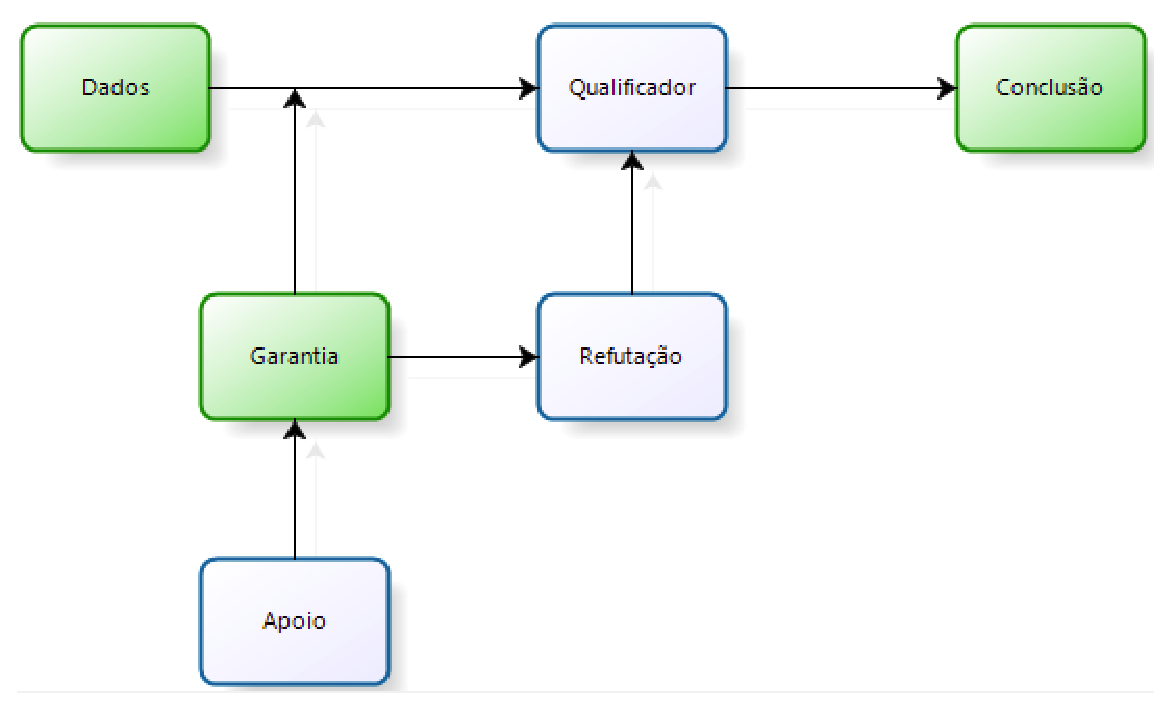
\includegraphics[width=0.9\textwidth]{elementos_modelo_toulmin}
\caption{Estrutura do Modelo de Toulmin.}
\label{elementos_modelo_toulmin}
\end{figure}

Com base na Figura \ref{elementos_modelo_toulmin}, os elementos com a cor verde são obrigatórios, enquanto que os elementos de cor azul são opcionais. Os dados representam as bases de raciocínio que suportam a conclusão. As informações implícitas que relacionam os dados e a conclusão são apresentadas através das garantias. Caso existam potenciais objeções à conclusão tomada, qualificadores podem ser definidos. Geralmente os qualificadores são inferidos a partir de determinadas restrições ou refutações não consideradas pelos dados e garantias do modelo. As refutações também podem ser relacionadas com garantias para aumentar sua autonomia. Os elementos de apoio oferecem justificativas para as garantias às tornando mais confiáveis.   Um exemplo da utilização do modelo de Toulmin é apresentado na Figura \ref{aplicacao_modelo_toulmin}.

\graphicspath{{figuras/}}
\begin{figure}[H]
\centering
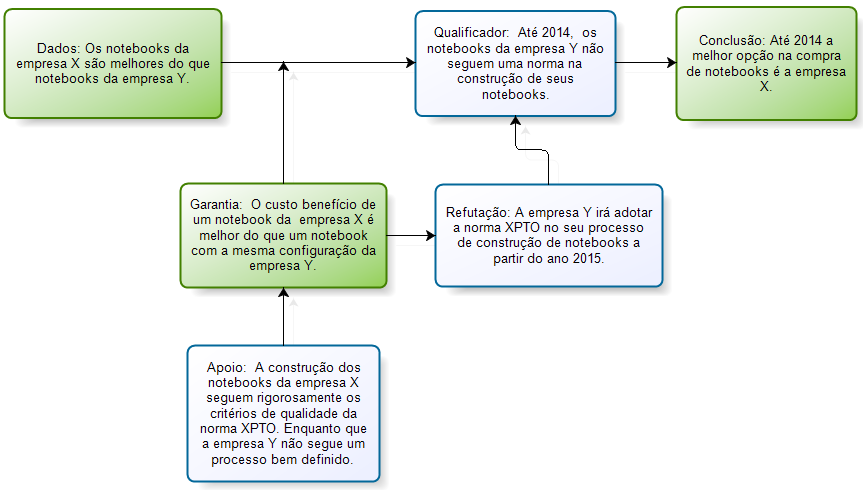
\includegraphics[width=0.9\textwidth]{aplicacao_modelo_toulmin}
\caption{Aplicação do Modelo de Toulmin.}
\label{aplicacao_modelo_toulmin}
\end{figure}

\citeonline{bentahar2010taxonomy} definiram um conjunto de vantagens e desvantagens existentes no modelo de Toulmin e suas extensões. Apresenta-se na Tabela \ref{tab-vd-toulmin} o resultado da análise realizada pelos autores, bem como percepções obtidas através da construção do exemplo apresentado na Figura \ref{aplicacao_modelo_toulmin}.

\begin{longtable}{|p{7cm}|p{7cm}|}
\caption{Avaliação do Modelo de Toulmin. }\\
\hline
\textbf{Vantagens} & \textbf{Desvantagens} \\
\hline
\endfirsthead
\multicolumn{2}{c}%
{\tablename\ \thetable\ -- \textit{Continuação da Página Anterior}} \\
\hline
\textbf{Vantagens} & \textbf{Desvantagens} \\
\hline
\endhead
\hline \multicolumn{2}{r}{\textit{Continua na Próxima Página}} \\
\endfoot
\hline
\endlastfoot
Considera diversos componentes de um argumento e os relacionamentos entre eles. & Relação entre os elementos da argumentação pode ser ambígua. O modelo é baseado em lógica informal. As regras de inferência podem não estar claras, permitindo argumentos duvidosos. \\ \hline
Permite a suposição de regras de inferência para deduzir conclusões acerca das premissas identificadas. & É complicado relacionar os diversos elementos de um argumento em um processo de argumentação. \\ \hline
Baseia-se em pilares filosóficos e empíricos. & O critério de aceitabilidade dos argumentos não é especificado. \\ \hline
Facilita a construção de argumentos textuais. & Tem como foco a estruturação dos argumentos. Os participantes da discussão e suas bases de conhecimento não são considerados. \\ \hline
Oferece suporte a elicitação de conhecimento. &  \\ \hline
Provê uma forma interessante de representar o conhecimento. & 
\label{tab-vd-toulmin}
\end{longtable}

\subsection{Framework IBIS}

O IBIS \footnote{Issue-Based Information System ou Sistemas de Informação Baseados em Questões} destina-se a coordenação e planejamento dos processos de tomada de decisões políticas. Este framework tem como objetivo estimular o raciocínio investigatório que facilita a identificação de argumentos. Ele auxilia na elaboração de questões a serem debatidas, na exploração de posições que responde estas questões e no suporte do processo de disputa entre os envolvido.

Como um modelo de estruturação de discursos, o IBIS auxilia o processo de comunicação em um domínio de resolução de problemas. Isso permite que o sistema capture diferentes aspectos do problema com base em diferentes pontos de vistas dos participantes da discussão. Assumindo diversos pontos de vistas para um determinado problema, aumenta a chance de aplicar uma solução consistente para resolvê-lo \cite{ebadi_collaborative_2009}. Os elementos fundamentais do framework IBIS são descritos na Tabela \ref{tab-elem-ibis}.

\begin{longtable}{|p{5cm}|p{9cm}|}
\caption{Elementos do Framework IBIS.}\\
\hline
\textbf{Elemento} & \textbf{Descrição} \\
\hline
\endfirsthead
\multicolumn{2}{c}%
{\tablename\ \thetable\ -- \textit{Continuação da Página Anterior}} \\
\hline
\textbf{Elemento} & \textbf{Descrição} \\
\hline
\endhead
\hline \multicolumn{2}{r}{\textit{Continua na Próxima Página}} \\
\endfoot
\hline
\endlastfoot
Questão & Representa o objeto alvo de discussão. Possui o formato de questões e tem origem acerca de temas controversos. \\ \hline
Posição & Representa uma resposta que soluciona uma questão. Espera-se que uma questão tenha várias posições. \\ \hline
Argumento & Representa uma relação de apoio ou oposição a determinada posição. A validade de uma posição é definida a partir dos argumentos a favor e contra.
 
\label{tab-elem-ibis}
\end{longtable}

O IBIS framework tem como meta a conexão das questões chaves de um problema. Cada questão pode ter diversas posições. Uma posição é uma afirmação ou asserção que resolve a questão. Geralmente as posições são independente uma das outras. Os argumentos são utilizados para oferecer suporte ou objeção às posições. Apresentam-se na Figura \ref{elementos_modelo_ibis} os possíveis relacionamentos entre os elementos do IBIS.

\graphicspath{{figuras/}}
\begin{figure}[H]
\centering
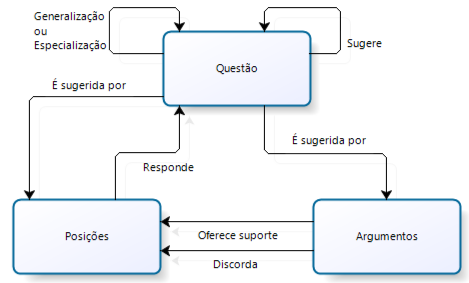
\includegraphics[width=0.7\textwidth]{elementos_modelo_IBIS}
\caption{Elementos do Framework IBIS.}{Adaptado de \cite{ebadi_collaborative_2009}} 
\label{elementos_modelo_ibis}
\end{figure}

Com base na Figura \ref{elementos_modelo_ibis}  é possível observar a flexibilidade do IBIS. As questões podem ser geradas a partir das informações presentes em posições, argumentos e, até mesmo, em outras questões. Vale destacar a representação macro do argumento, contrapondo a representação interna proposta pelo modelo de Toulmin. Apresenta-se na Figura \ref{aplicacao_modelo_ibis}  um exemplo da aplicação do IBIS. Neste exemplo serão descritos alguns aspectos estruturais exibindo as características fundamentais deste framework.

\graphicspath{{figuras/}}
\begin{figure}[H]
\centering
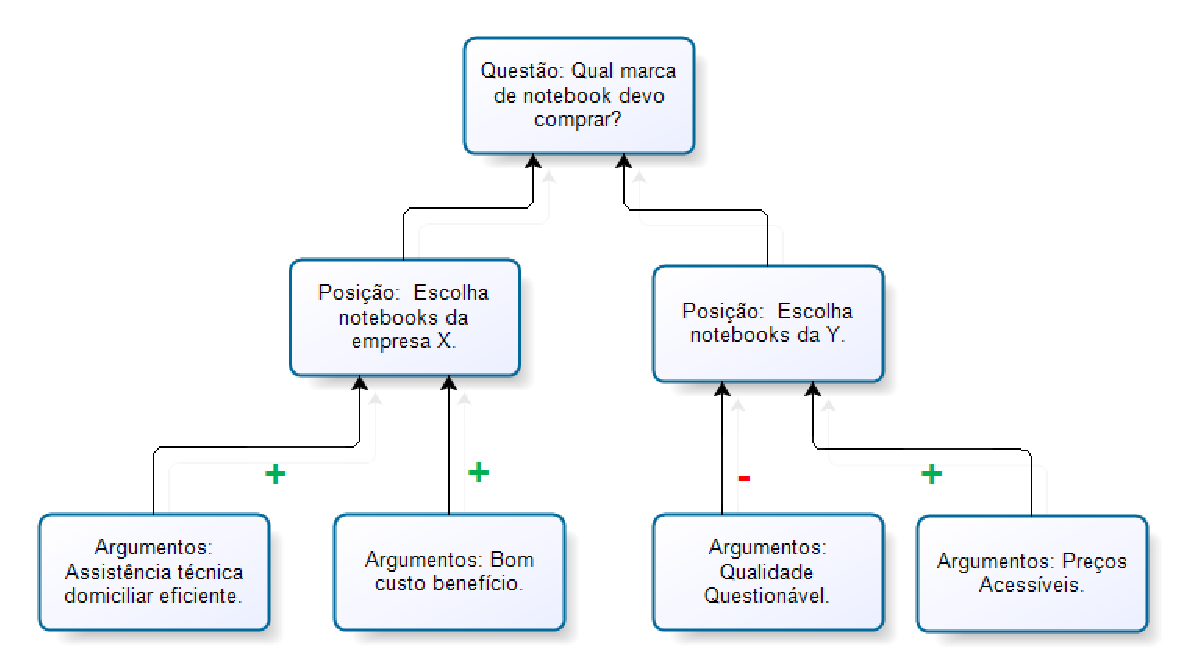
\includegraphics[width=0.7\textwidth]{aplicacao_modelo_ibis}
\caption{Aplicação do Framework IBIS.} 
\label{aplicacao_modelo_ibis}
\end{figure}

O exemplo apresentado na Figura \ref{aplicacao_modelo_ibis} descreve uma discussão para determinar qual marca de notebook um participante deve comprar. O objeto alvo de discussão é interpretado como uma questão. Os pontos de vistas dos participantes da discussão são convertidos para as estruturas genéricas chamadas posições. Para finalizar, argumentos a favor ou contra cada posição são estabelecidos. Ao término do modelo, as decisões podem ser feitas com base em critérios bem definidos e o diagrama resultante pode ser documentado para facilitar a rastreabilidade das decisões tomadas.

A partir dos trabalhos de \citeonline{ebadi_collaborative_2009}, \citeonline{guerrero2002decision}, \citeonline{conklingibis1988} e \citeonline{Kunz1970issuesas}, uma análise envolvendo as vantagens e desvantagens do IBIS foi realizada. O resultado desta análise é apresentado na Tabela \ref{tab-vd-ibis}. 

\begin{longtable}{|p{7cm}|p{7cm}|}
\caption{Avaliação do Framework IBIS.}\\
\hline
\textbf{Vantagens} & \textbf{Desvantagens} \\
\hline
\endfirsthead
\multicolumn{2}{c}%
{\tablename\ \thetable\ -- \textit{Continuação da Página Anterior}} \\
\hline
\textbf{Vantagens} & \textbf{Desvantagens} \\
\hline
\endhead
\hline \multicolumn{2}{r}{\textit{Continua na Próxima Página}} \\
\endfoot
\hline
\endlastfoot
Permite a captura de diferentes aspectos do problema tendo como base pontos de vistas diferentes. Aumenta a probabilidade de seleção da melhor solução para uma questão específica. & Os participantes leigos neste framework têm dificuldades para classificar se um determinado conceito é uma questão, posição ou argumento. \\ \hline
Os três elementos básicos do modelo permitem a representação de qualquer atividade deliberativa. & Regras rígidas para a construção de um diagrama. Um argumento não pode ser o vértice inicial de uma discussão. \\ \hline
Aumenta a qualidade do diálogo, pois os participantes estão focados nas questões definidas. & Precisa de regras semânticas para facilitar a realização de inferências. Não possui um ponto de parada que represente o fim da discussão. \\ \hline
Aumenta a transparência do processo de tomadas de decisões. Os participantes podem rastrear os motivos que levaram uma determinada decisão. & A análise de diagramas contendo uma discussão extensa não é trivial. O grafo resultante pode dificultar a análise da argumentação.
\label{tab-vd-ibis}
\end{longtable}

\subsection{Framework de Argumentação Abstrato}

Em 1995, P. M. Dung apresentou um framework de argumentação abstrato \cite{dung1995321} com uma série de regras semânticas para avaliar a aceitabilidade dos argumentos. Em resumo, o framework proposto por Dung pode ser visualizado como um grafo direcionado contendo vértices que representam os argumentos e arestas que representam as relações binárias de ataque entre os argumentos \cite{Brewka2014}. Os argumentos são entidades abstratas e não possuem uma estrutura interna em particular.

O framework de Dung é definido formalmente pelo par \textit{F = (A, R)}. Onde que o A representa o conjunto de elementos abstratos chamados argumentos e o R representa as relações binárias entre estes argumentos. A seguir será realizado um exemplo demonstrando estes conceitos. Considere a seguinte argumentação a respeito da escolha de um notebook:

\begin{itemize}

\item A1: O notebook da empresa X possui desempenho superior a um notebook da empresa Y com a mesma configuração. Assim, certamente é o melhor custo benefício.

\item A2: O notebook da empresa Y é mais barato do que o seu concorrente na empresa X. Assim, apesar de possuir desempenho menor, é o melhor custo benefício.

\item A3: A qualidade das peças utilizadas na construção do notebook da empresa X são superiores as peças utilizados na construção dos notebooks da empresa Y. A vida útil do notebook da empresa X será maior do que o do concorrente. 

\item A4: Apesar de barato, vários consumidores estão reclamando do notebook da empresa Y devido a problemas de aquecimento.

\end{itemize}

Apresenta-se na Figura \ref{aplicacao_framework_dung} a argumentação acerca da escolha de um notebook seguindo as diretrizes do framework de Dung. As setas representam as relações de ataque. Nesta discussão, \textit{A = {A1, A2, A3, A4}} e \textit{R = {(A1 > A2), (A2 > A1), (A3 > A2), (A4 > A2)}}. Vale ressaltar que um argumento que não foi atacado está aceito. Caso contrário, estará derrotado se nenhum outro argumento da discussão estiver defendendo o mesmo. O argumento que está atacando é válido apenas se estiver aceito. Caso dois argumentos aceitos ataquem um ao outro, uma situação de indefinição irá ocorrer. Para evitar esta situação, mais informações significantes devem ser adicionadas ao grafo da discussão.

\graphicspath{{figuras/}}
\begin{figure}[H]
\centering
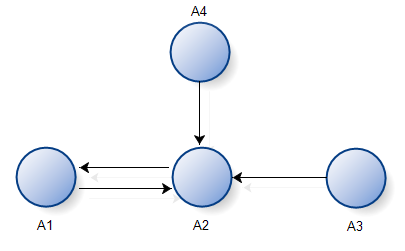
\includegraphics[width=0.7\textwidth]{aplicacao_framework_dung}
\caption{Aplicação do Framework de Dung.} 
\label{aplicacao_framework_dung}
\end{figure}

A partir do exemplo definido na Figura \ref{aplicacao_framework_dung}, dois conceitos fundamentais relacionados à aceitabilidade dos argumentos podem ser aplicados: O \textbf{conjunto livre de conflitos} representa um agrupamento de argumentos que não se atacam; \textbf{O conjunto admissível} é um conjunto livre de conflitos que defende-se de ataques de argumentos pertencentes a outras extensões. O conjunto \textit{S = {A1, A3, A4}} é um conjunto admissível livre de conflitos.
 
As semânticas utilizadas para verificar a aceitabilidade dos argumentos possibilitam diferentes formas de raciocínio. Elas produzem subconjuntos de argumentos válidos chamados extensões. Uma argumentação pode possuir várias extensões. Apresenta-se na Tabela \ref{tab-semantica-dung} semânticas definidas no framework.

\begin{longtable}{|p{4cm}|p{9cm}|}
\caption{Semânticas do Framework de Dung.}\\
\hline
\textbf{Semântica} & \textbf{Descrição} \\
\hline
\endfirsthead
\multicolumn{2}{c}%
{\tablename\ \thetable\ -- \textit{Continuação da Página Anterior}} \\
\hline
\textbf{Semântica} & \textbf{Descrição} \\
\hline
\endhead
\hline \multicolumn{2}{r}{\textit{Continua na Próxima Página}} \\
\endfoot
\hline
\endlastfoot
Crédula (Credulous) & A maior extensão de argumentos válidos é selecionada. A extensão resultante é chamada de Extensão Preferida (Preferred Extension). \\ \hline
Cética (Sceptical) & A menor extensão de argumentos válidos é selecionada. A extensão resultante é chamada de Extensão Fundamentar (Grounded Extension).  \\ \hline
Estável (Stable) & Uma extensão é dita estável caso ele derrote qualquer argumento que não pertença a ele. A extensão resultante é chamada de Extensão Estável (Stable Extension).

\label{tab-semantica-dung}
\end{longtable}

Aplicando as semânticas disponíveis no framework ao exemplo da Figura \ref{aplicacao_framework_dung} obtém-se sempre o mesmo resultado. A discussão possui apenas uma extensão de argumentos admissível. Caso a argumentação possuísse várias extensões admissíveis, a análise ficaria da seguinte forma: Aplicando a semântica crédula resultaria no conjunto com o número máximo de argumentos aceitos; Aplicando a semântica cética resultaria no conjunto com o número mínimo de argumentos aceitos; Aplicando a semântica estável resultaria em todos os conjuntos que atacam todos os argumentos externos que não pertencem a ele.

A partir dos trabalhos de \citeonline{dung1995321}, \citeonline{Modgil2013}, \citeonline{maudet2007}, \citeonline{zhang_temporal_2012}, \citeonline{prakken09anabstract} e \citeonline{Brewka2014}, uma análise envolvendo as vantagens e desvantagens do framework foi elaborada. Apresenta-se na Tabela \ref{tab-vd-dung} o resultado desta análise.

\begin{longtable}{|p{7cm}|p{7cm}|}
\caption{Avaliação do Framework de Dung.}\\
\hline
\textbf{Vantagens} & \textbf{Desvantagens} \\
\hline
\endfirsthead
\multicolumn{2}{c}%
{\tablename\ \thetable\ -- \textit{Continuação da Página Anterior}} \\
\hline
\textbf{Vantagens} & \textbf{Desvantagens} \\
\hline
\endhead
\hline \multicolumn{2}{r}{\textit{Continua na Próxima Página}} \\
\endfoot
\hline
\endlastfoot
Notação simples e intuitiva. Estruturar a discussão em um grafo é uma tarefa trivial. Pois os argumentos são representados como vértices e existe apenas um relacionamento entre eles, a relação de ataque. & Relação de preferência entre argumentos em conflito não foi definida. \\ \hline
A aceitabilidade dos argumentos pode ser interpretada a partir de um ponto de vista cético, crédulo ou estável. & A relação de ataque entre argumentos é binária. Grupos de argumentos não podem realizar ou sofrer ataques. \\ \hline
Analisa a aceitabilidade dos argumentos de uma forma abstrata. Não considera estrutura interna, origem ou concepção dos argumentos. &  \\ \hline
Semântica formal permitindo a adoção da abordagem em sistemas computacionais. & 
 
\label{tab-vd-dung}
\end{longtable}

\subsection{Framework ACE}

O ACE \footnote{Acceptability Evaluation ou Avaliação da Aceitabilidade} \cite{jureta2009AMA} é um framework de argumentação baseado em proposições que possui origem na engenharia de requisitos. Este framework oferece maneiras de modelar e raciocinar acerca da validação relativa dos requisitos discutidos em uma reunião. A validação relativa pode ser vista como um consenso dos participantes de uma discussão a respeito de um artefato. O framework é composto de uma linguagem para representar as informações extraídas de uma discussão, uma condição de aceitabilidade para verificar a existência de consenso entre os participantes e procedimentos para checar a condição de aceitabilidade automaticamente.

Os modelos de argumentação, gerados com base na linguagem contida no ACE, são grafos direcionados com rótulos.  Os vértices são classificados com base em quatro rótulos: i, It, P e C. Os vértices com rótulo (i) representam vértices de informação que servem de entrada ou saída para inferências (It). Os vértices com o rótulo (I) representam a aplicação de inferências a fim de obter determinadas saídas. Os vértices com rótulo (C) representam regras de conflito envolvendo dois ou mais vértices em um grafo. Finalmente, os vértices com rótulo (P) representam regras de preferência envolvendo a predileção de dois ou mais vértices do grafo. As arestas do grafo possuem apenas um rótulo (To).

Apresenta-se na Figura \ref{aplicacao_framework_ace} um exemplo da aplicação da linguagem ACE. O exemplo modela uma discussão envolvendo uma provável aquisição de notebooks por parte de uma empresa. O grafo da discussão contem três proposições i(p1), i(p2) e i(p3) descritas a seguir:

\begin{itemize}

\item i(p1): Comprar um notebook da marca X oferece um bom custo benefício. Isto é essencial para empresa que esta enfrentando dificuldades financeiras.

\item i(p2): O notebook da marca nacional X possui preço acessível e boa qualidade em suas peças.

\item i(p3): Alguns notebooks nacionais da marca X apresentam defeitos após um ano de uso. É interessante adquirir notebooks da marca internacional Y. Apesar de mais caros, a qualidade do produto compensa a diferença de preços.

\end{itemize}

A proposição i(p2) foi inferida a partir de uma regra indutiva tendo como insumo i(p1). Com base nas ideias expressas em i(p1) pode-se inferir que o “bom custo-benefício representa um produto com qualidade e acessível no contexto da empresa que está enfrentando problemas financeiros. Porém,  a  proposição i(p3) contrapõe as ideias apresentadas em i(p1) exibindo argumentos contra a aquisição de notebooks de marcas nacionais. A relação de inferência entre as proposições i(p1) e i(p2) é descrita formalmente como \textit{It(i(p1),i(p2))}. Enquanto que a relação de conflito envolvendo i(p3) e i(p2) é definida formalmente como \textit{C1(i(p3),i(p2))}. Para finalizar, supõe-se que um questionário tenha sido aplicado na empresa e os funcionários preferiram os notebooks nacionais da marca X aos importados da marca Y. O vértice P1 representa uma regra de preferência entre as proposições i(p2) e i(p3). O uso da preferência gera um conflito \textit{C2(P1, {C1,i(p3)})} que protege a proposição i(p3). A preferência é definida formalmente como \textit{P1(i(p2),i(p3))}.

\graphicspath{{figuras/}}
\begin{figure}[H]
\centering
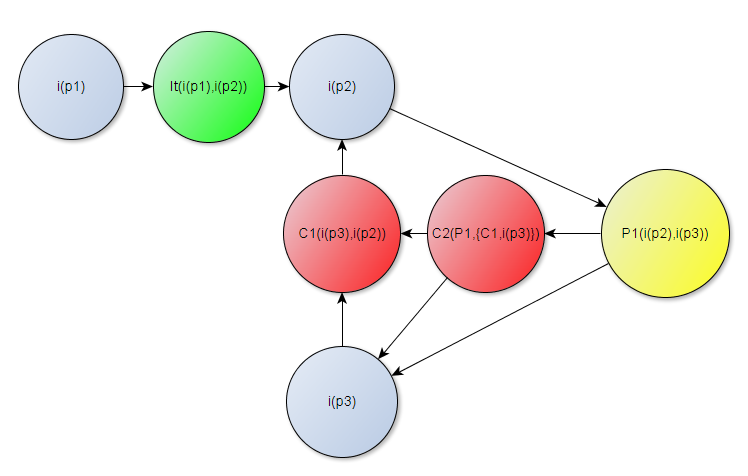
\includegraphics[width=0.7\textwidth]{grafo_ace}
\caption{Aplicação do Framework ACE.} 
\label{aplicacao_framework_ace}
\end{figure}

A aceitabilidade proposta pelo ACE é baseada em três rótulos: A, AD e R. O rótulo A (Accepted) determina que um vértice do grafo foi aceito. O rótulo AD (Accepted and Dominated) é utilizado para representar vértices aceitos, porém, em uma relação de preferência, não foram priorizados. Finalmente, o rótulo R (Rejected) representa vértices que foram rejeitados por intermédio de um conflito. Com base nestes rótulos, cada vértice do grafo é computado individualmente.

Para definir a aceitabilidade de um vértice são executadas duas tarefas fundamentais: recuperação e avaliação. A tarefa de recuperação oferece uma rotina para identificar sub grafos com informações relevantes para a elaboração da condição de aceitabilidade de um vértice. O algoritmo de recuperação é baseado em uma busca em largura (BFS). Através da aplicação deste algoritmo é possível identificar todos os caminhos do grafo que terminam no vértice que está sendo avaliado. Já a tarefa de avaliação é mais complexa. segue uma descrição do processo de execução desta tarefa:

\begin{itemize}

\item Identificar os componentes fortemente conectados (SCC) do grafo de discussão;

\item Definir o ordenamento topológico dos componentes fortemente conectados. Resultando em um grafo direcionado acíclico (DAG).

\item Computar os rótulos A, AD e R para cada SCC do grafo. Para essa rotina existem duas abordagens:

\begin{itemize}
\item SCC sem ciclos: Primeiramente, deve-se rotular tendo como base as posições definidas na ordenação topológica. Logo em seguida, o SCC que não contenha linhas de encontro é selecionado e rotulado. Os componentes já rotulados são ignorados, permitindo que o ciclo de rotulação continue nos outros componentes do DAG.

\item SCC com ciclos: Primeiramente, deve-se realizar a contagem n de  todos os ciclos existentes no SCC. Logo após, todos os vértices do ciclo recebem o rótulo A. A partir do último vértice adicionado ao SCC, n agentes irão percorrer e rotular os vértices de todos os caminhos possíveis até retornarem ao vértice inicial e rotulá-lo em conjunto. Uma sequência de rótulos de avaliação é gerada para cada vértice.  O critério de parada é atingindo quando os dois últimos rótulos do vértice inicial são iguais. Nesta situação, a aceitabilidade de cada vértice é definida como sendo o último elemento da sequência de rótulos. Caso essa condição não seja satisfeita, os agentes serão enviados novamente até que a sequência do vértice inicial possua quatro rótulos. Persistindo a diferença entre os dois últimos rótulos do vértice inicial, a aceitabilidade se torna inconclusiva. A adição de informações relevantes será necessária para a avaliação da aceitabilidade. 

\end{itemize}
\end{itemize}	
	
Apresenta-se na Figura \ref{aceitabilidade_framework_ace} a avaliação da aceitabilidade do vértice i(p2) a partir da discussão definida na Figura \ref{aplicacao_framework_ace}.

\graphicspath{{figuras/}}
\begin{figure}[H]
\centering
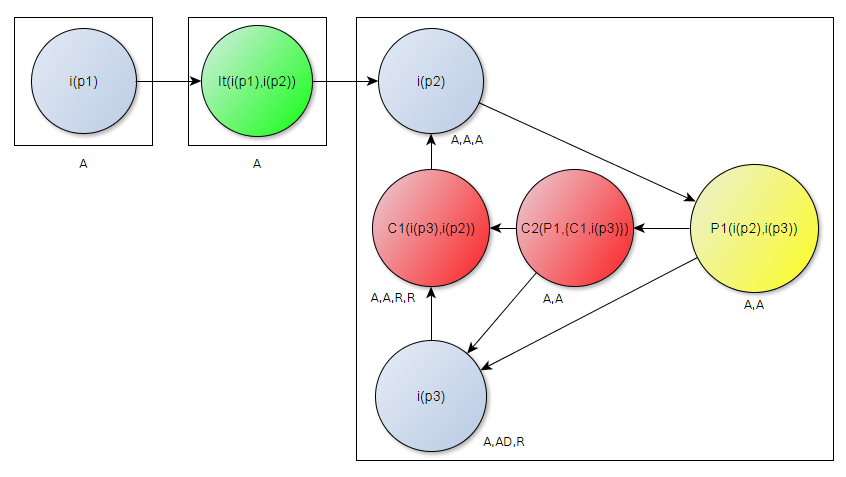
\includegraphics[width=1\textwidth]{graph_ace_evaluation}
\caption{Avaliação da Aceitabilidade do Framework ACE.} 
\label{aceitabilidade_framework_ace}
\end{figure}

Ao término da avaliação da aceitabilidade do vértice i(p2), observa-se que todos os vértices relacionados também foram avaliados. Apenas o conflito C1 e a proposição i(p3) foram rejeitados. As regras bem como os algoritmos utilizados para computar os rótulos A, AD e R nos vértices de um grafo estão disponíveis em anexo.

Com base no trabalho de \cite{jureta2009AMA} e nos exemplos desenvolvidos na Figura \ref{aplicacao_framework_ace} e \ref{aceitabilidade_framework_ace}, apresenta-se na Tabela \ref{tab-vd-ace} as vantagens e desvantagens do framework ACE.

\begin{longtable}{|p{7cm}|p{7cm}|}
\caption{Avaliação do Framework ACE.}\\
\hline
\textbf{Vantagens} & \textbf{Desvantagens} \\
\hline
\endfirsthead
\multicolumn{2}{c}%
{\tablename\ \thetable\ -- \textit{Continuação da Página Anterior}} \\
\hline
\textbf{Vantagens} & \textbf{Desvantagens} \\
\hline
\endhead
\hline \multicolumn{2}{r}{\textit{Continua na Próxima Página}} \\
\endfoot
\hline
\endlastfoot
Define uma condição de aceitabilidade que determina a validação relativa de um artefato. & Usuários leigos no contexto da argumentação podem ter problemas para entender os relacionamentos entre os elementos do grafo. \\ \hline
A linguagem oferecida é simples e expressiva. Facilitando a representação dos  elementos presentes em uma discussão. & Não foi encontrada nenhuma ferramenta computacional que se baseie neste framework. \\ \hline
Provê algoritmos para a recuperação e avaliação dos argumentos de uma discussão. &   
 
\label{tab-vd-dung}
\end{longtable}

\section{Argumentação na Web}

Diversas áreas de pesquisa tais como inteligência artificial, filosofia, linguística e engenharia de software estão propondo diferentes abordagens que compreendem técnicas de argumentação. O interesse na argumentação é evidente, porém as diferentes abordagens desenvolvidas consideram aspectos específicos do domínio de aplicação. Isto acaba dificultando a integração e unificação dos resultados de cada proposta em um modelo de argumentação geral e coerente \cite{bex_formal_2010}. Estas várias abordagens dificultam a integração dos dados gerados a partir das  ferramentas computacionais que auxiliam o processo de argumentação e geralmente não ofertam técnicas para lidar com a lógica da argumentação \cite{rahwan2011}.  

Para solucionar os problemas acima, uma linguagem de marcação chamada AIF\footnote{Argument Interchange Format ou Formato para a Troca de Argumentos} \cite{rahwan2011} foi elaborada. O AIF consiste de uma ontologia que unifica conceitos semelhantes que são utilizados na argumentação em vários contextos. Os principais objetivos do AIF são: facilitar a troca de informações entre ferramentas que suportam o processo de argumentação; simplificar o desenvolvimento de sistemas multiagentes, principalmente na racionalidade dos agentes inteligentes. 
	
O AIF pode ser dividida em duas ontologias:  superior e formal. A ontologia superior define uma linguagem contendo diversos elementos para representar uma discussão. A ontologia formal oferece uma série de padrões que auxiliam a análise racional dos argumentos de um discurso.  Os padrões podem variar dependendo do contexto que ocorre o diálogo. Apresenta-se na Figura \ref{elementos-ontologia-aif} a estrutura geral e os relacionamentos dos conceitos presentes no AIF. 

\graphicspath{{figuras/}}
\begin{figure}[H]
\centering
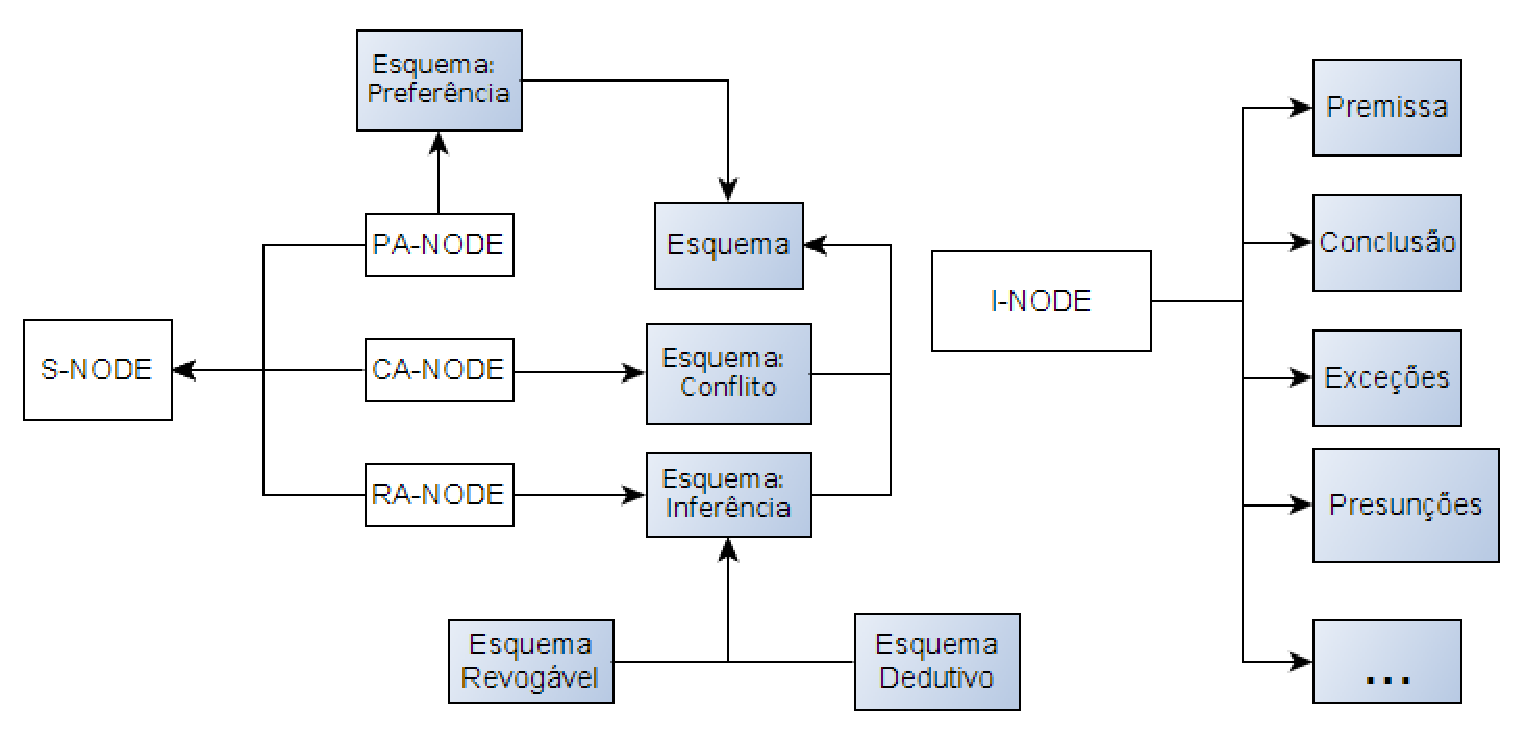
\includegraphics[width=1\textwidth]{aif_ontologia_2}
\caption{Estrutura da Ontologia AIF.}{Adaptado de \cite{bex_formal_2010}} 
\label{elementos-ontologia-aif}
\end{figure}

Com base na Figura \ref{elementos-ontologia-aif}, observa-se que a ontologia define quatro tipos de nó. Os nós \textit{I-NODE}\footnote{Information Node ou Nó de Informação} encapsulam as informações disponíveis na discussão. Estas informações podem possuir caráter dedutível: premissas ou conclusões, ou revogável: presunções ou exceções. Os nós de informação representam a base de conhecimento concebida como conseqüência de uma discussão. Os nós \textit{S-NODE}\footnote{Scheme Node ou Nó de Esquema} representam aplicações de esquemas, ou seja, padrões racionais. A partir deles, regras de inferência, preferência e conflito podem ser estabelecidas. Os esquemas de argumentação podem ser classificados. O esquema de inferência foi classificado em duas diretrizes diferentes: \textit{Dedutivo} e \textit{Revogável}. O esquema dedutivo compreende aspectos relacionados a lógica formal. Esta abordagem consiste no processo de gerar conclusões a partir de premissas válidas de forma monotônica. Já o esquema revogável considera a lógica não monotônica, ou seja, a adição de novas informações, confiáveis ou não, pode modificar o resultado de uma ou várias conclusões. 

Apresenta-se na Figura \ref{aplicacao_aif} um exemplo de aplicação do AIF. O exemplo consiste de uma discussão envolvendo a venda de um notebook. Os nós de informação e de esquema são representados, respectivamente, pela cor azul e laranja. Os nós de esquema são gerados a partir de percepções lógicas baseadas nas informações presentes na discussão. As informações são apresentados a seguir:

\begin{itemize}

\item \textit{I1} João garante para José que o notebook está sem problemas.
\item \textit{I2} O notebook está sem problemas.
\item \textit{I3} O notebook está funcionando corretamente.
\item \textit{I4} José ouviu falar que João não é confiável.
\item \textit{I5} João afirma que é confiável.
\item \textit{PA1} Por meio de uma pesquisa com seus amigos, José descobriu que João é confiável.  

\end{itemize}

\graphicspath{{figuras/}}
\begin{figure}[H]
\centering
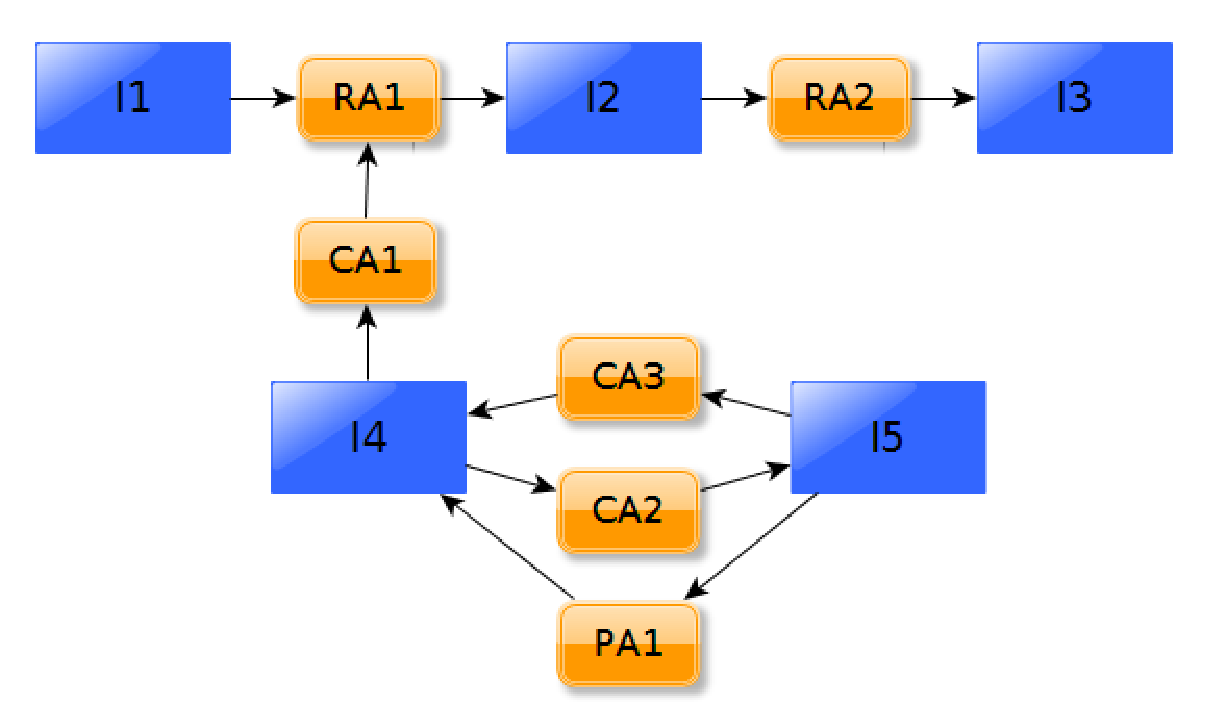
\includegraphics[width=1\textwidth]{aplicacao_aif}
\caption{Aplicação da Ontologia AIF.} 
\label{aplicacao_aif}
\end{figure}

O nó de informação \textit{I2} foi gerado através de uma regra de inferência \textit{RA1} revogável, as premissas que oferecem suporte para I2 possuem certas restrições. O conflito \textit{CA1}, gerado a partir do nó \textit{I4}, está atacando \textit{RA1}. A conclusão \textit{I2} é válida por conta da aplicação de uma regra de preferência \textit{PA1} que apoia o nó \textit{I5}, contrário ao nó \textit{I4}. Para finalizar, uma conclusão pode servir de insumo para uma nova regra de inferência. O nó \textit{I3} foi gerado por intermédio da regra de inferência dedutiva \textit{RA2}, que teve como insumo a conclusão \textit{I2}.
  